\documentclass[a4paper,12pt]{article}
\usepackage{HomeWorkTemplate}
\usepackage{circuitikz}
\usepackage[shortlabels]{enumitem}
\usepackage{float}
\usepackage{hyperref}
\usepackage{tikz}
\usepackage{amsmath}
\usepackage{amssymb}
\usepackage{tcolorbox}
\usepackage{xepersian}
\settextfont{XB Niloofar}
\usetikzlibrary{arrows,automata}
\usetikzlibrary{circuits.logic.US}
\usepackage{changepage}
\newcounter{problemcounter}
\newcounter{subproblemcounter}
\setcounter{problemcounter}{1}
\setcounter{subproblemcounter}{1}
\newcommand{\problem}[1]
{
	\subsection*{
		پرسش
		\arabic{problemcounter} 
		\stepcounter{problemcounter}
		\setcounter{subproblemcounter}{1}
		#1
	}
}
\newcommand{\subproblem}{
	\textbf{\harfi{subproblemcounter})}\stepcounter{subproblemcounter}
}


\begin{document}
\handout
{آز طراحی سیستم‌های دیجیتال}
{دکتر سیاوش بیات سرمدی}
{نیم‌سال اول 1400\lr{-}1401}
{اطلاعیه}
{پرهام چاوشیان}
{98100118}
 {گزارش آزمایش سوم}
{خانم زینب رشیدی}
\textbf{بخش اول: }
ماژول
$one\_bit\_comparator$
ماژول $cascadable$ای است که برای مقایسه دو بیت استفاده می‌شود. این ماژول به این صورت کار می‌کند که باتوجه به خروجی‌های ماژول قبلی و بیت‌های ورودی برای خروجی تصمیم‌ می‌گیرد. اگر ماژول قبلی، خروجی بزرگتر یا کوچکتر داده باشد، خروجی ماژول را بزرگتر یا کوچکتر می‌کند. اگر ماژول قبلی، مساوی اعلام کرده باشد، بسته به اینکه بیت‌ها ورودی چه وضعیتی دارند، نتیحه را اعلام می‌کند. منظور از بزرگتر یا کوچکتر، بزرگتر یا کوچکتر بودن بیت $a$ از بیت $b$ است. در ماژول
$comparator$
یک پارامتر
$number\_of\_bits$
داریم که تعداد بیت‌های اعداد ورودی را مشخص می‌کند و به صورت پیشفرض برابر 4 است. همچنین با استفاده از $generate$ سوال را در حالت کلی حل می‌کنیم. از سه بردار برای ذخیره کردن مقادیر میانی بزرگتر، کوچکتر یا تساوی مقایسه‌کننده‌ها استفاده می‌کنیم. درواقع، در کد ما به تعداد بیت‌ها مقایسه کننده تولید می‌کنیم که این بردارها به نوعی سیم‌های واصل بین این مقایسه‌کننده‌ها وهمچنین حاوی ورودی و خروجی اولین و آخرین مقایسه کننده هستند.\\
نتایج شبیه‌سازی نیز در ادامه آمده است (در صورت نیاز تصاویر به طور جداگانه نیز پیوست شده اند):
\begin{figure}[H]
 \centering
  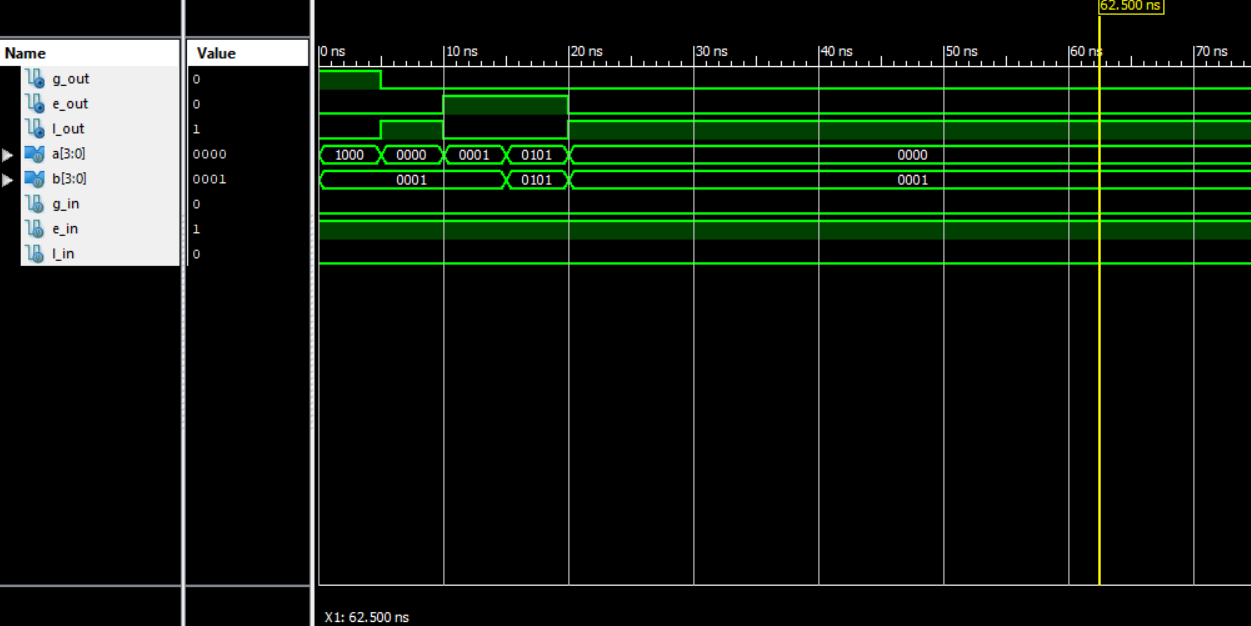
\includegraphics[width=0.8\linewidth]{s1}
\end{figure}
\textbf{بخش دوم: }
در این بخش ما در واقع از 3 عدد $DFF$ استقاده کرده‌ایم، اما از آنجایی که در صورت ازمایش ذکر شده است که تنها باید یک ماژول داشته باشیم، ماژول جداگانه‌ای برای $DFF$ در نظر نگرفتیم. همچنین مطابق با مطالب کلاس، فرض بر این بوده است که بیت‌ها از کم‌ارزش به پرارزش ورودی داده ‌می‌شوند. با این فرض در هر گام بسته به اینکه بیت‌های ورودی فعلی چه هستند، و همچنین بسته به اینکه نتیجه مقایسه قبلی چه بوده است، مقادیر نتیجه جدید را تولید می‌کند. البته در تعیین مقادیر جدید خروجی به فعال یا غیرفعال بودن ریست نیز توجه شده است. بعد از اینکه مقادیر جدید خروجی تعیین شد، به کمک $DFF$هایی که داشتیم، با لبه بالارونده کلاک، مقادیر به روز می‌شوند.\\
نتایج شبیه‌سازی نیز در ادامه آمده است (در صورت نیاز تصاویر به طور جداگانه نیز پیوست شده اند):
\begin{figure}[H]
 \centering
  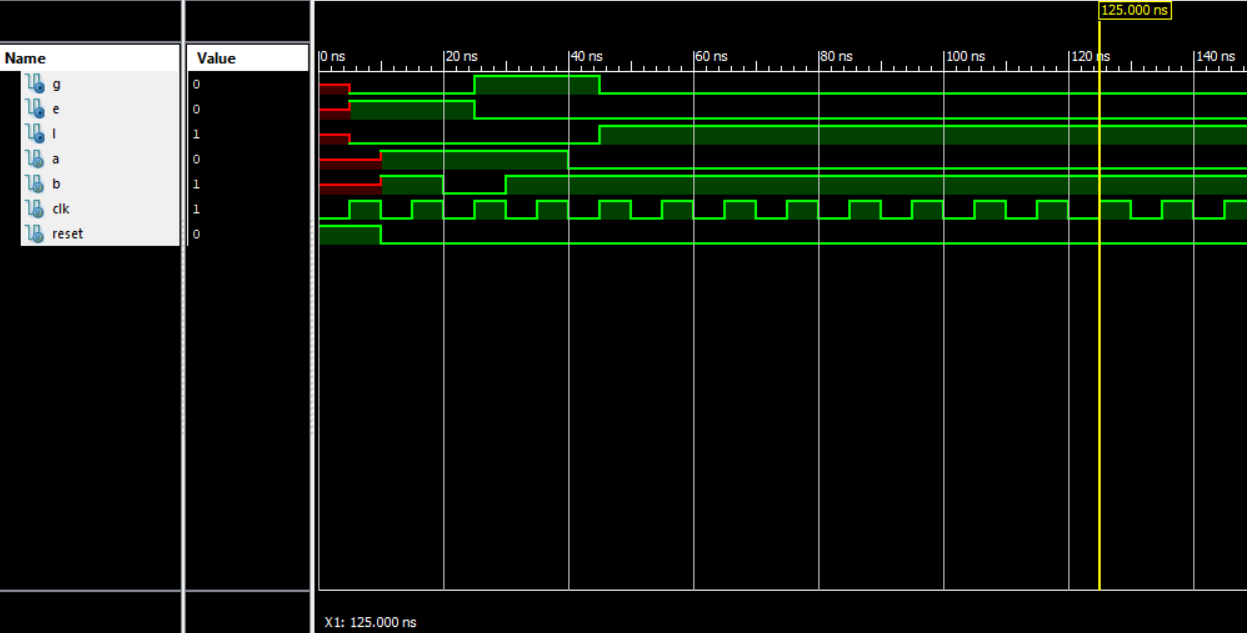
\includegraphics[width=0.8\linewidth]{s2}
\end{figure}
\end{document}